

\chapter[Naslov poglavlja u sadržaju][Kratki naslov poglavlja]{Naslov poglavlja}	
% ukoliko naslov nije jako dugacak dovoljno je samo \chapter{Naslov poglavlja} 

\section[Naslov sekcije u sadržaju][Kratki naslov sekcije]{Naslov sekcije}
\subsection{Naslov podsekcije}
\begin{thm}
Iskaz teorema u kojem se javljaju skupovi  $\N$, $\Z$, $\Q$, $\R$ i $\C$.
\end{thm}
\begin{conj}
Iskaz slutnje u kojoj se javljaju funkcije $\tg$, $\tgh$ i $\sh$.
\end{conj}
\begin{cor}
Iskaz posljedice u kojoj se javljaju skupovi $\Ker T$ i $\slika T$..
\end{cor}
\begin{proof}
Dokaz posljedice se nalazi u \cite{kljuc}. Pogledajte i \cite{kurepa1956convex}, \cite{kurepa1981funkcionalna} te \cite{Dutkay:2009}.
\end{proof}SDGFSFDG


SDGSDG  sdfsfg f fdh fgj gh jgjk jkj k yk k klk l fs fd gsdfg dfh dfghj fj ghjk gjk jlk sdf 
$x_1+x_2+x_3+x_4=12$ $x_1+x_2+x_3+x_4=12$
 $x_1+x_2+x_3+x_4=12$ $x_1+x_2+x_3+x_4=12$ $x_1+x_2+x_3+x_4=12$ $x_1+x_2+x_3+x_4=12$
 $x_1+x_2+x_3+x_4=12$ $x_1+x_2+x_3+x_4=12$ $x_1+x_2+x_3+x_4=12$
$x_1+x_2+x_3+x_4=12$ 
SDGSG sdfsfg f fdh fgj gh jgjk jkj k yk k klk l fs fd gsdfg dfh dfghj fj ghjk gjk jlk sdf sfdh j fj tuk ugad h j yrtu iru i
\[ z \left( 1 \ +\ \sqrt{\omega_{i+1} + \zeta -\frac{x+1}{\Theta +1} y + 1}
\ \right) =  1 \]

GSDFGSDFG



\begin{equation}
\label{eq:jed1}
	1+1=2
\end{equation}

SDG
SDFGS
SDGSFG

\label{stranica}
Na stranici \pageref{stranica} se nalaza slika u \textbf{png} formatu.
% slike smiju biti u svim formatima koje podrzava pdf (pdf, jpg, png)
\begin{figure}[h!t]
\begin{center}

\includegraphics[scale=0.5]{mosaic-from-pompeii.png}
\caption{Prva slika}
\end{center}
\end{figure}

Na slici \ref{fig:3d} se nalazi 3D graf neke funkcije. 

\begin{figure}[h!t]
\centering 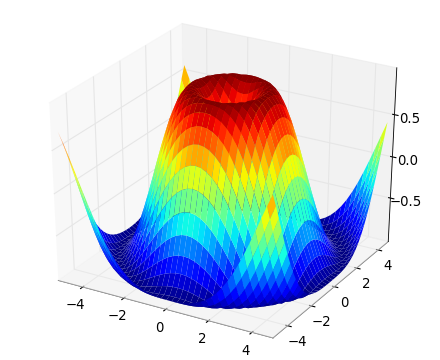
\includegraphics{surface3d.png}
\caption{Druga slika}
\label{fig:3d}
\end{figure}

kao i jedna vrlo komplicirana formula koja slijedi iz \eqref{eq:jed1}
\[ \sum_{i=1}^{\infty}A_{x_1}\times A_{{\alpha}_2}\oslash\iint_{\Omega}x^2\ddagger\limsup_{n\in\N}\frac{\alpha+\theta+\gamma}{n^{\omega}}\;\;\text{je u stvari}\;\;\biguplus_{r\in\Q}\overline{\Xi_i \mathop\Theta_{\substack{j\in\C \\ j\ni i\Q}} \Upsilon^{k^j} \underset{\ast}{\Psi} \hslash\vert_{\{\alpha\}}}.\]
